
%(BEGIN_QUESTION)
% Copyright 2006, Tony R. Kuphaldt, released under the Creative Commons Attribution License (v 1.0)
% This means you may do almost anything with this work of mine, so long as you give me proper credit

Explain why this {\it 4-wire} RTD circuit is completely immune to calibration drift resulting from cable resistance:

$$\includegraphics[width=15.5cm]{i00415x01.eps}$$

Also, identify the magnitude and polarity of all voltage drops in this circuit.

\vskip 20pt \vbox{\hrule \hbox{\strut \vrule{} {\bf Suggestions for Socratic discussion} \vrule} \hrule}

\begin{itemize}
\item{} How will the temperature measurement be affected if the current source's value is increase?
\item{} Will this circuit be immune to calibration drift even if the RTD wire resistances are not all equal to each other?  Is this true for a three-wire RTD circuit as well?
\item{} Explain the meaning of the DC source symbol used in this diagram.  What type of source is this, and what is its polarity?
\item{} Choose a resistor at random in this circuit and imagine that it fails (either open or shorted).  Would this electrical fault make the RTD appear hotter than it really is, or colder than it really is?  Explain your answer in detail.
\end{itemize}

% CHANGE THIS TO A FAULT ANALYSIS QUESTION???

\underbar{file i00415}
%(END_QUESTION)





%(BEGIN_ANSWER)

%(END_ANSWER)





%(BEGIN_NOTES)

$$\includegraphics[width=15.5cm]{i00415x02.eps}$$

\vfil \eject

$$\includegraphics[width=15.5cm]{i00415x03.eps}$$

\vskip 20pt \vbox{\hrule \hbox{\strut \vrule{} {\bf Virtual Troubleshooting} \vrule} \hrule}

This question is a good candidate for a ``Virtual Troubleshooting'' exercise.  Presenting the diagram to students, you first imagine in your own mind a particular fault in the system.  Then, you present one or more symptoms of that fault (something noticeable by an operator or other user of the system).  Students then propose various diagnostic tests to perform on this system to identify the nature and location of the fault, as though they were technicians trying to troubleshoot the problem.  Your job is to tell them what the result(s) would be for each of the proposed diagnostic tests, documenting those results where all the students can see.

During and after the exercise, it is good to ask students follow-up questions such as:

\begin{itemize}
\item{} What does the result of the last diagnostic test tell you about the fault?
\item{} Suppose the results of the last diagnostic test were different.  What then would that result tell you about the fault?
\item{} Is the last diagnostic test the best one we could do?
\item{} What would be the ideal order of tests, to diagnose the problem in as few steps as possible?
\end{itemize}

%INDEX% Measurement, temperature: RTD (4-wire with cable resistance)

%(END_NOTES)


